\medskip
\hfill
\begin{minipage}[t]{.45\textwidth}
  \textbf{$\LWE_{n,q,\chi}$ problem:}\\Given $m \geq 1$, $\mathbf{A} \sample \mathcal U(\Zq^{n \times m})$,\\
  $\textcolor{orange!70!black}{\mathbf{e}} \sample \chi^m$ \\[.5em]
  $\left(
    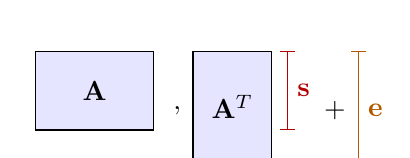
\begin{tikzpicture}
      \tikzstyle{matA}=[fill=blue!10]
      \tikzstyle{vecS}=[color=red!70!black]
      \tikzstyle{vecE}=[color=orange!70!black]
      \path[use as bounding box] (-2.1, .5) rectangle (2.4, 1.8);
      \draw[matA, xshift=-2cm, yshift=.5cm] (0,0) rectangle node {$\mathbf{A}$} (1.5,1);
      \node at (-.2, .75) {$,$};
      \draw[matA] (0,0) rectangle node {$\mathbf{A}^T_{}$} (1,1.5);
      \draw[|-|, vecS] (1.2, 1.5) -- node[right] {$\mathbf{s}$} ++(0, -1);
      \node at (1.8, .75) {$+$};
      \draw[|-|, vecE] (2.1, 1.5) -- node[right] {$\mathbf{e}$} ++ (0, -1.5);
    \end{tikzpicture}
  \right)$\\[.5em]
  $\in \Zq^{n \times m} \times \Zq^{m}$,
  find $\textcolor{red!70!black}{\mathbf{s}} \in \Zq^n.$
\end{minipage} \hfill
\begin{minipage}[t]{.4\textwidth}
  \textbf{$\SIS_{n,m,q,\beta}$ problem:}\\Given\\[.5em]
  $\tikz[baseline=.3cm]{ \draw[fill=blue!10] (0,0) rectangle node {$\mathbf{A}$} (1.5,1); } \in \Zq^{n \times m},$
  find $\textcolor{red!70!black}{\mathbf{x}} \in \ZZ^m_{}$ such that\\[.5em]
  $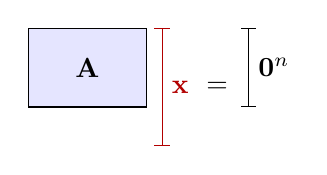
\begin{tikzpicture}[baseline=.25cm]
    \tikzstyle{matA}=[fill=blue!10]
    \tikzstyle{vecX}=[color=red!70!black]
    \draw[matA] (0,0) rectangle node {$\mathbf{A}$} (1.5,1);
    \draw[|-|, vecX] (1.7, 1) -- node[right] {$\mathbf{x}$} ++ (0, -1.5);
    \node at (2.4, .25) {$=$};
    \draw[|-|] (2.8, 1) -- node[right] {$\mathbf{0}^n$} ++ (0, -1);
  \end{tikzpicture},$ and\\$0< \|\textcolor{red!70!black}{\mathbf{x}}\| \leq \beta$.
\end{minipage}
\hfill
\medskip

